% Flowchart
% Author: Stefan Kottwitz
% https://www.packtpub.com/hardware-and-creative/latex-cookbook
\documentclass[border=20pt]{standalone} 
%%%<
\usepackage{verbatim}
%%%>
\begin{comment}
:Title: Flowchart
:Tags: Charts;Flowcharts;Cookbook
:Author: Stefan Kottwitz
:Slug: math-flowchart

A flowchart showing how we may choose a math
environment.

It shows using styles, placing nodes in a matrix,
and drawing arrows using loops.
\end{comment}
\usepackage[a4paper,vmargin=3cm]{geometry}
\usepackage{tikz}
\usetikzlibrary{matrix,calc,shapes}
\tikzset{
  treenode/.style = {shape=rectangle, rounded corners,
                     draw, anchor=center,
                     text width=5em, align=center,
                     top color=white, bottom color=blue!20,
                     inner sep=1ex},
  decision/.style = {treenode, diamond, inner sep=0pt},
  root/.style     = {treenode, font=\Large, bottom color=red!30},
  env/.style      = {treenode, font=\ttfamily\normalsize},
  finish/.style   = {root, bottom color=green!40},
  dummy/.style    = {circle,draw}
}
\newcommand{\yes}{edge node [above] {yes}}
\newcommand{\no}{edge  node [left]  {no}}
\begin{document}
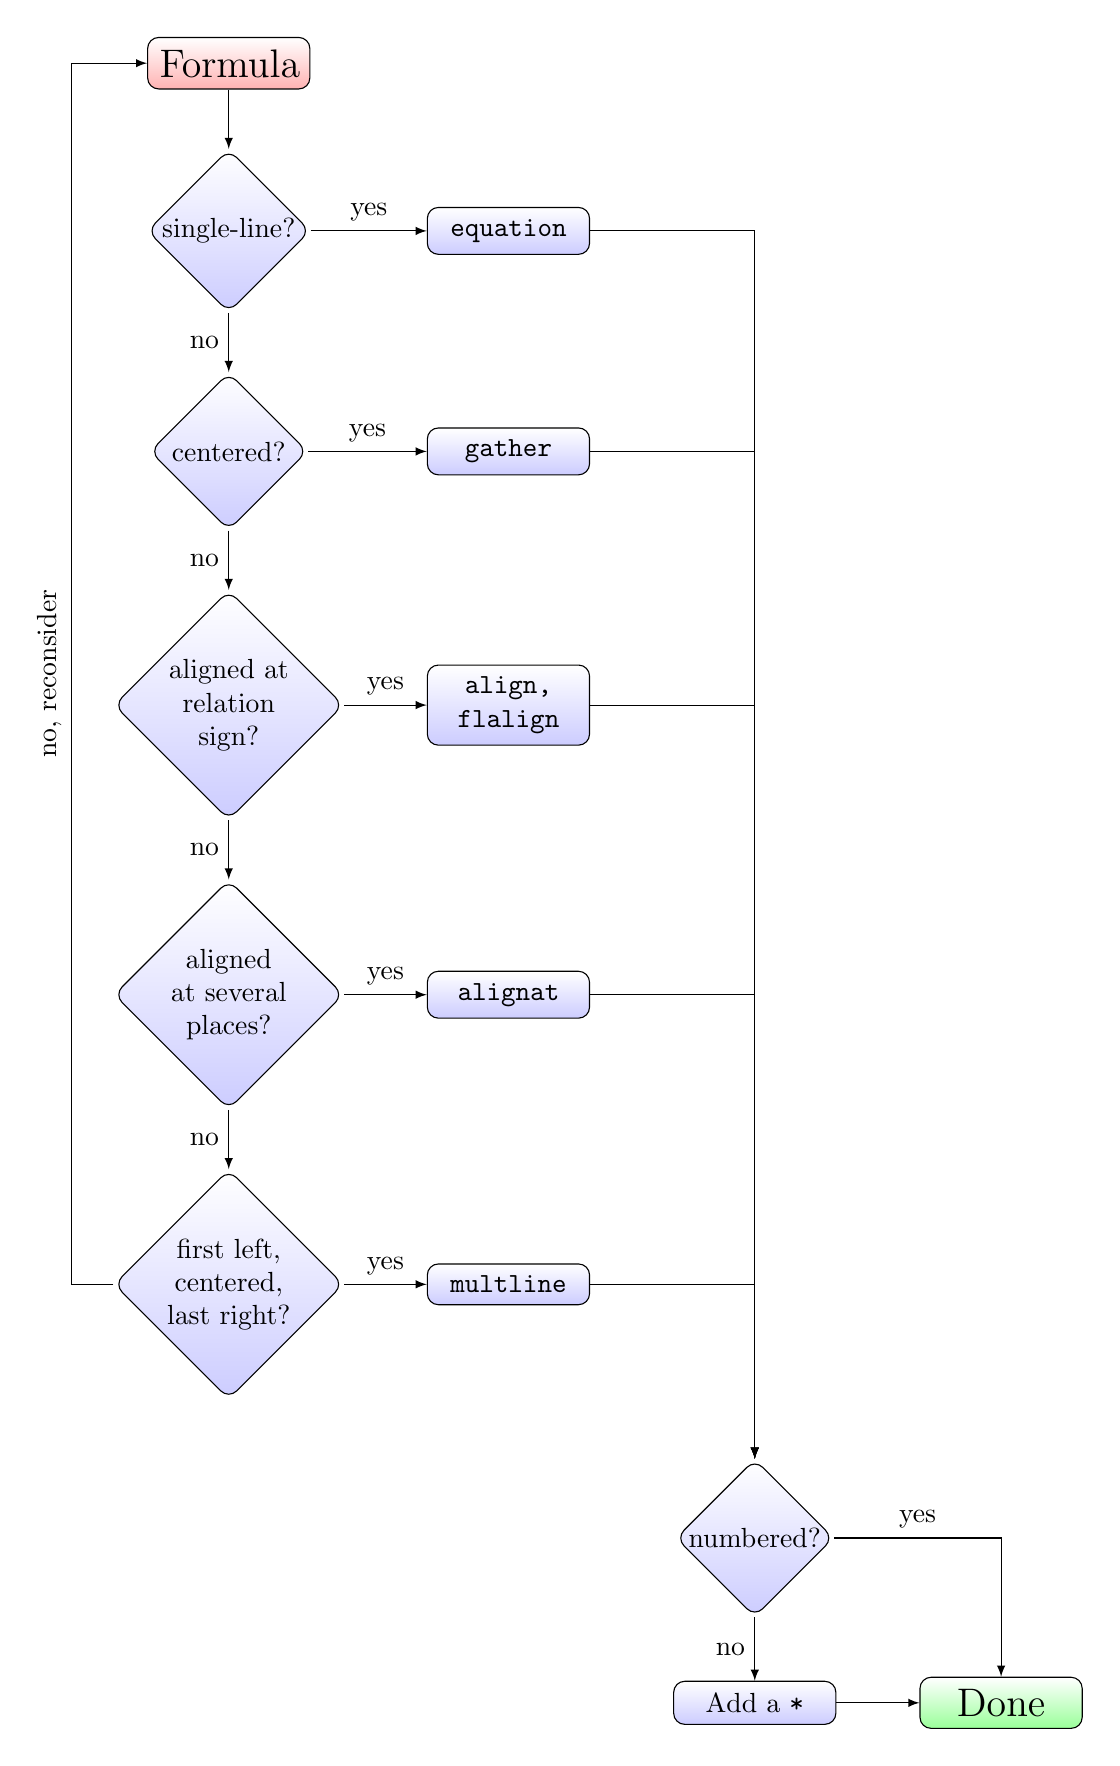
\begin{tikzpicture}[-latex]
  \matrix (chart)
    [
      matrix of nodes,
      column sep      = 3em,
      row sep         = 5ex,
      column 1/.style = {nodes={decision}},
      column 2/.style = {nodes={env}}
    ]
    {
      |[root]| Formula           &                \\
      single-line?               & equation       \\
      centered?                  & gather         \\
      aligned at relation sign?  & align, flalign \\
      aligned at several places? & alignat        \\
      first left, centered,
        last right?              & multline       \\
      & & |[decision]| numbered? \\
      & & |[treenode]| Add a \texttt{*} & |[finish]| Done \\
    };
  \draw
    (chart-1-1) edge (chart-2-1)
    \foreach \x/\y in {2/3, 3/4, 4/5, 5/6} {
      (chart-\x-1) \no (chart-\y-1) }
    \foreach \x in {2,...,6} {
       (chart-\x-1) \yes (chart-\x-2) }
   (chart-7-3) \no  (chart-8-3)
   (chart-8-3) edge (chart-8-4);
 \draw
   (chart-6-1) -- +(-2,0) |- (chart-1-1)
     node[near start,sloped,above] {no, reconsider};
  \foreach \x in {2,...,6} {
   \draw (chart-\x-2) -| (chart-7-3);}
 \draw   (chart-7-3)  -| (chart-8-4)
   node[near start,above] {yes}; 
\end{tikzpicture}
\end{document}
